\documentclass[a4paper,twoside,twocolumn,10pt]{article}
\usepackage{abstract} % Style for abstracts in Dept. CSIS, OPU
%\usepackage{abstract4past} % Style for abstracts for the past curriculum

%%%%%%%%%% Designate packages you need %%%%%%%%%%
\usepackage[dvipdfmx]{graphicx} % Enhanced support for graphics
\usepackage{url} % Verbatim with URL-sensitive line breaks


%%%%%%%%%% Parameters that should be customized %%%%%%%%%%
% Language (1 = Japanese, 2 = English)
\setlang{1}
% Bachelor or Master (1 = Bachelor, 2 = Master)
\setborm{1}
% Fiscal year
\setfy{2018}
% Group number
\setgnum{1}
% Presentation order
\setorder{4}
% Increase page number (optional)
%% \pplus{1}

% Title
\title{機械学習を用いた麻雀戦術における状況予測手法の提案}
% Author
\author{青野 義樹}
%%%%%%%%%% Parameters that should be customized (end) %%%%%%%%%%

\begin{document}
\maketitle % Insert title
\small

\section{はじめに}
近年,機械学習や深層学習の手法に基づく,ゲームをプレイする人工知能プログラムが盛んに開発されている.本研究では不完全情報ゲームの 1 種である麻雀を対象とした.

麻雀では,あるプレイヤが捨てた牌の種類や捨てた順番などから,そのプレイヤが現在手持ちにしている牌の状態の予測が可能である.この予測は戦術構築の際に重要であり,一般的に上級者ほどその予測精度は高いと考えられている.水上らの研究 \cite{pre_stu} では,ロジスティック回帰と線形回帰を用いたモデルが人間の上級者と同程度の予測精度を得ているが,モデルの単純さや特徴量の設計などの面から,局面中の複雑な特徴を十分に捉えて予測しているとはいえない.そこで本研究では,Recurrent Neural Network (RNN) の一種である Long Short-Term Memory (LSTM) によるニューラルネットワークモデルを用いて,捨てた牌の時系列的な特徴を捉えることで予測精度の向上を試みる.

\section{麻雀の用語とゲーム進行について}
以下に麻雀のゲーム進行と用語について説明する.

麻雀は 4 人のプレイヤによってプレイされる.1 ゲームは局と呼ばれる単位によって区切られている.局の始めに,各プレイヤはそれぞれ 13 枚の牌を手持ちにしており, 1 枚手持ちに加える行為と, 1 枚手持ちから捨てる行為を繰り返すことで牌を入れ替えていく.牌の組合せで 3 枚の組 4 セットと 2 枚の組 1 セットという特定の条件を満たすことでアガリとなり,アガったプレイヤが点を得て局が終了する.局を複数回 (通常 8 回程度) 繰り返すことで 1 ゲームが終了する.1 ゲームの終了時に最も得点の多いプレイヤの勝利となる.
また,局の最中,プレイヤは他プレイヤがどの種類の牌を何枚手持ちにしているか直接知ることはできず,この点から麻雀には不完全情報性があるといえる.
\begin{itemize}
\item 鳴き\\
他プレイヤが捨てた牌を利用して自身の手持ち牌をアガリへ近付ける行為.%通常は,1 回の鳴きで他プレイヤが捨てた牌 1 枚と自身の手持ち牌 2 枚を組み合わせて 3 枚の組を 1 セット作る.作った 1 セットは,他プレイヤからも観測可能である.プレイヤ 1 人につき 1 局あたり 4 回まで鳴くことが可能である.

\item テンパイ\\
アガリの一つ手前の状態.%あと 1 枚必要な牌を加えることでアガリとなる.
他プレイヤの捨てた牌や鳴いた牌の情報などからそのプレイヤの手持ち牌がテンパイ状態にあるかの予測をテンパイ予測という.

\end{itemize}

\section{数値実験}
以下に,テンパイ予測の実験方法を示す.用いたデータはオンライン麻雀サイトの対戦ログファイルから,特定の局面のデータを取り出したものである.学習には $2.8\times10^6$ 個のデータを,テストには $6.0\times10^4$ 個のデータをそれぞれ用いた.

実験は局面中のある 1 人のプレイヤを対象にした.上記の局面のデータの内,そのプレイヤの捨てた牌,鳴いた牌,リーチをかけているかなどの情報から学習に用いる入力の素性ベクトルと出力のラベルを生成した.具体的には,捨てた牌 1 枚を 19 次元の特徴量ベクトルで表した.捨てた牌全体は,ルール上の捨てた牌の最大枚数に合わせて $19\times24$ 次元の行列で表した.鳴いた牌も同様に,1 セットを 14 次元の特徴量ベクトルで表し,鳴いた牌全体を $14\times4$ 次元の行列で表した.入力の素性ベクトルには,これらの行列と局面中のその他の情報を表すベクトルを用いた.出力のラベルには,対象プレイヤがテンパイしているかしていないかを表す 2 クラスを用いた.

用いたモデルの構成を以下に示す.まず入力層の次の層で,捨てた牌のデータと鳴いた牌のデータをそれぞれ異なる 2 つの LSTM 層で処理する.その次の層で,LSTM 層の 2 つの出力ベクトルとその他の入力情報ベクトルを結合する.得られたベクトルを Multi-Layer Perceptron (MLP) の入力とし,MLP の出力をモデルの出力とする.

\subsection{実験結果と考察}
図 \ref{result_tenpai} に実験の結果得られた ROC 曲線を示す.表 \ref{auc_tenpai} に図 \ref{result_tenpai} 中の各曲線の曲線下面積を示す.各図表中の model は本研究で作成したモデル,previous\_study は従来研究の論文中のモデルを本研究と同じデータを用いて再現したモデル,random は一様乱数によってテンパイと非テンパイを出力するランダムなモデルである.表 \ref{auc_tenpai} で示した曲線下面積は 1 に近いほどモデルが高精度であることを示す.本研究のモデルは従来研究のモデルおよびランダムなモデルと比較して高精度であることがわかる.

また,本研究で用いた特徴量は 514 次元であり,従来研究の特徴量の 6,888 次元と比較して約 7.5\% 程度であるため,特徴量ベクトルの次元数を大幅に削減できたといえる.

\begin{figure}[tb]
  \centering
  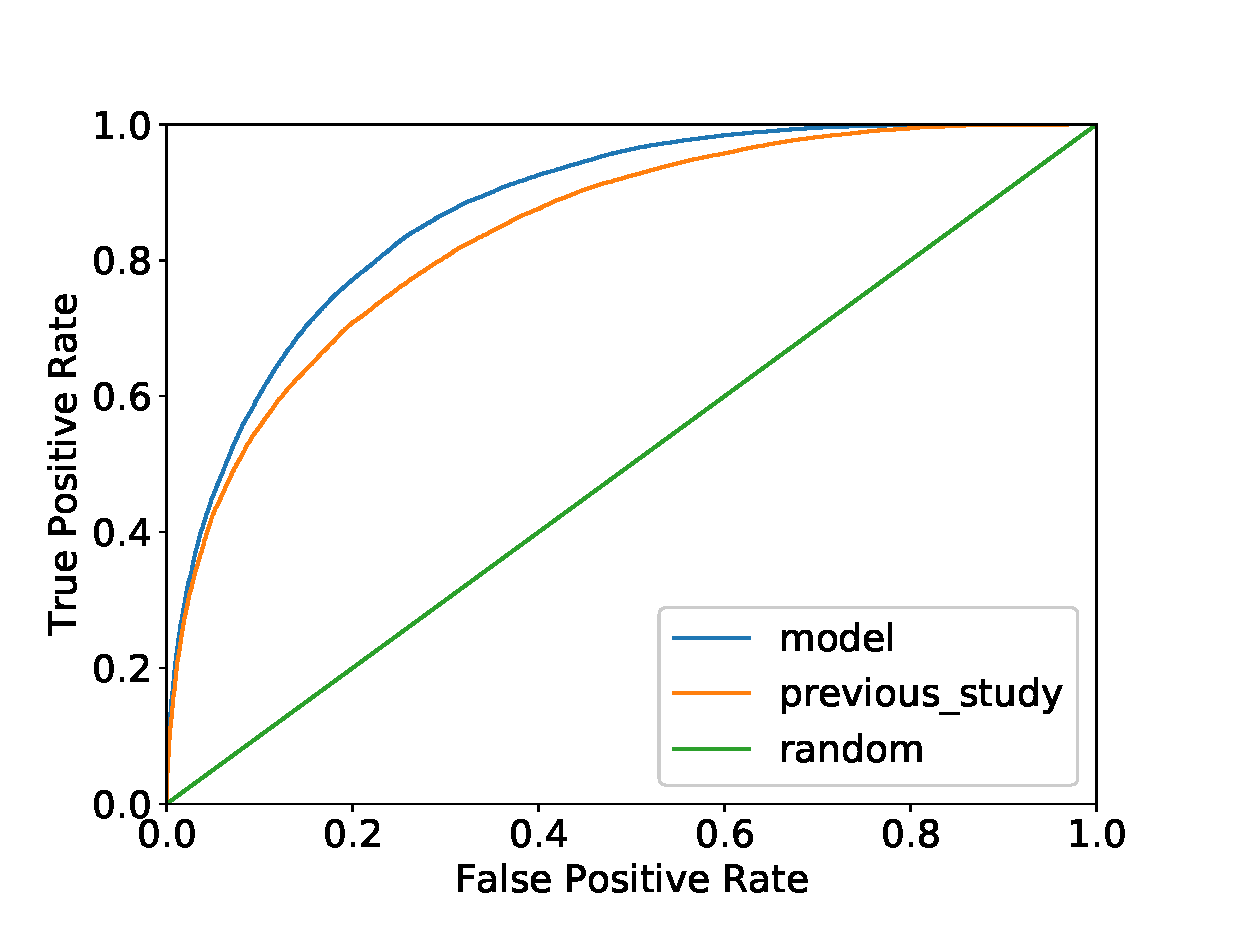
\includegraphics[width=7cm]{ROC_gather_nontitle.eps}
  \caption{テンパイ予測の ROC 曲線}
  \label{result_tenpai}
\end{figure}

\begin{table}[tb]
  \caption{ROC 曲線の曲線下面積}
  \label{auc_tenpai}
  \centering
  \begin{tabular}{|c||c|} \hline
  モデル & 曲線下面積 \\ \hline \hline
  model & 0.8761\\ \hline
  previous\_study & 0.8430\\ \hline
  random & 0.5000\\ \hline
  \end{tabular}
\end{table}
\section{まとめと今後の課題}
本研究では,LSTM によるニューラルネットワークモデルを用いて,従来よりも高精度な他プレイヤのテンパイ予測モデルを構築した.今後の課題としては,今回構築したモデルの予測結果を踏まえた上で最適な捨て牌を決定するモデルの構築が挙げられる.

%%%%%%%%%%%%%%%%%%%%%%%%%%%%%%

\bibliographystyle{jabbrvunsrt}
\bibliography{index_ja}
\end{document}
